\begin{columns}[totalwidth=.9\textwidth]
    \column{.75\textwidth}
        \begin{itemize}
            \item クラックの進展を\alert{抑制}
            \item Andrews 理論\footnote{
                \small{Andrews, E. H. and Fukahori, Y., J. of Mat. Sci. 12, 1307 (1977)}
            }
                \begin{itemize}
                    \item クラックの応力場
                    \item クラック進展時に、{\color{red} エネルギー散逸}
                    \item \alert{ヒステリシスに由来}
                \end{itemize}	
        \end{itemize}
    \column{.24\textwidth}
        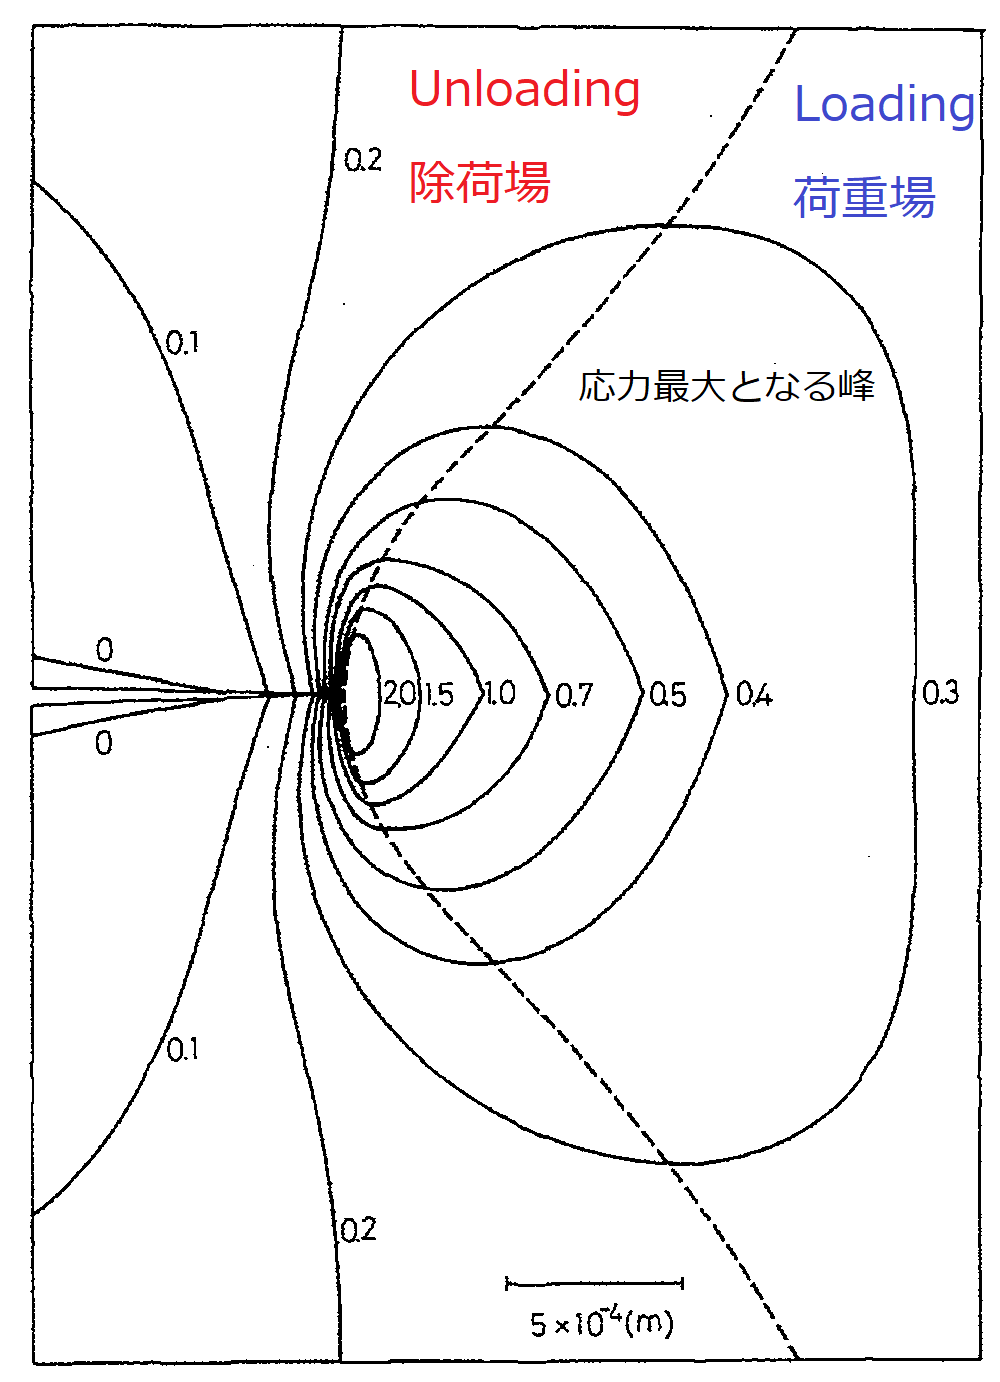
\includegraphics[width=.9\textwidth]{crack.png}     
\end{columns}
% \begin{alertblock}{疲労破壊も考慮すると}
%     \begin{itemize}
%         \item \alert{可逆的}であることが望ましい。\textcolor{blue}{$\neq$ 犠牲結合}
%         \item 変形の周期に対応できるように、\alert{回復速度}も重要。
%     \end{itemize}
% \end{alertblock}